\documentclass{article}
\usepackage[utf8]{inputenc}
\usepackage[T2A]{fontenc}
\usepackage{amsmath}
\usepackage{faktor} 
\usepackage{mathrsfs}
\usepackage[english,russian]{babel}
\usepackage{amssymb}
\usepackage{mathtools}
\usepackage{amsthm}
\usepackage{float}
\usepackage[shortlabels]{enumitem}
\usepackage[left=2cm,right=2cm, top=2cm,bottom=2cm,bindingoffset=0cm]{geometry}

\DeclareMathOperator{\ord}{ord}
\DeclareMathOperator{\orb}{Orb}
\DeclareMathOperator{\stab}{Stab}
\DeclareMathOperator{\lcm}{lcm}
\DeclareMathOperator{\inn}{Inn}
\DeclareMathOperator{\Ker}{Ker}
\DeclareMathOperator{\im}{Im}
\DeclareMathOperator{\tr}{tr}
\DeclareMathOperator{\rk}{rk}
\DeclareMathOperator{\interior}{int}
\DeclareMathOperator{\conv}{conv}
\DeclareMathOperator{\dom}{dom}
\DeclareMathOperator*{\argmax}{arg\,max}
\DeclareMathOperator*{\argmin}{arg\,min}
\DeclareMathOperator{\diag}{diag}
\DeclareMathOperator{\cone}{cone}
\DeclareMathOperator{\sign}{sign}
\DeclareMathOperator{\rint}{rint}
\DeclareMathOperator{\aff}{aff}

\newcommand*{\QED}{\null\nobreak\hfill\ensuremath{\square}}
\newcommand*{\R}{\mathbb{R}}
\newcommand*{\st}{\text{s.t. }}
\newcommand*{\1}{\mathbf{1}}

\title{ККТ and duality}
\author{Ковалев Алексей}
\date{}

\begin{document}

\maketitle

\paragraph{1.}
\[ \begin{split}
    x^2 + 1 &\to \min\limits_{x \in \R} \\
    \st (x - 2)&(x - 4) \leqslant 0
\end{split} \]
Feasible set -- $[2; 4]$, минимум функции равен $p^\ast = 5$, достигается на $x^\ast = 2$.
\[ L(x,\, \lambda) = x^2 + 1 + \lambda (x - 2)(x - 4) \]
\[ g(\lambda) = \inf\limits_{x \in R} L(x,\, \lambda) \]
В силу выпуклости лагранжиана получаем, что $\inf\limits_{x \in R} L(x,\, \lambda)$ достигается на $x^\ast :\: \nabla_x L(x^\ast,\, \lambda) = 0$. 
\[ 2x^\ast + \lambda (2 x^\ast - 6) = 0 \]
Тогда двойственная задача
\[ \begin{split}
    \frac{9 \lambda^2}{(1 + \lambda)^2} + 1 - \lambda \cdot \frac{(\lambda - 2)(\lambda + 4)}{(1 + \lambda)^2} &\to \max\limits_{\lambda \in \R} \\
    \st & \lambda \geqslant 0
\end{split} \]
Вогнутость этой задачи непосредственно проверяется дифференциальным критерием выпуклости первого порядка при $\lambda \geqslant 0$. Также из условия $\nabla g(\lambda^\ast) = 0$ получаем, что $\lambda^\ast = 2,\, d^\ast = 5$, то есть сильная двойственность присутствует.

\noindent
Красным на рисунке $x^2 + 1$, зеленым, фиолетовым, черным -- лагранжиан при разных $\lambda$ (1, 2, 7 соответственно)
\begin{figure}[H]
    \centering 
    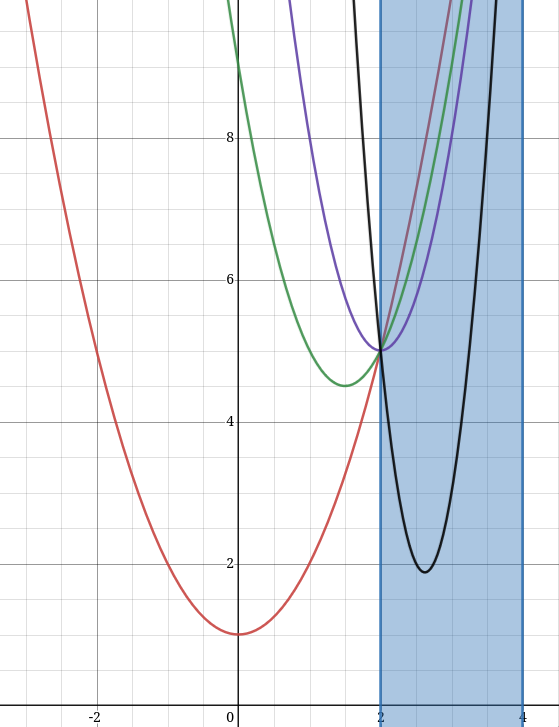
\includegraphics[scale=0.4]{graph.png}
\end{figure}


\paragraph{2.} $ A \in \R^{m \times n},\, b \in \R^m,\, \lambda > 0. $ 
\[ \begin{split} 
    \frac{1}{2} \| y - b \|_2^2 + \frac{\lambda}{2} \|x\|_2^2 &\to \min\limits_{x \in \R^n,\, y \in \R^m} \\ 
    \st & y = Ax \end{split} \]
\[ L(x,\, y,\, \mu) = \frac{1}{2}\|y - b\|_2^2 + \frac{\lambda}{2}\|x\|_2^2 + \mu^{\top} (y - Ax) \]
\[ g(\mu) = \inf\limits_{x \in \R^n,\, y \in \R^m} L(x,\, y,\, \mu) \]
$L(x,\, y,\, \mu)$ -- выпуклая по $x$ и $y$ функция. Значит $\inf\limits_{x \in \R^n,\, y \in \R^m} L(x,\, y,\, \mu)$ достигается при $x^\ast,\, y^\ast$, таких что $\nabla_{(x, y)} L(x^\ast,\, y^\ast,\, \mu) = 0$.
\[ \nabla_x L(x^\ast,\, y^\ast,\, \mu) = \lambda x^\ast - A^\top \mu = 0;\; \nabla_y L(x^\ast,\, y^\ast,\, \mu) = y^\ast - b + \mu = 0 \]
\[ g(\mu) = \frac12 \|\mu\|_2^2 + \frac{1}{2\lambda} \|A^\top \mu\|_2^2 + \mu^\top \left(b - \mu - \frac{1}{\lambda} AA^\top \mu\right) \]
\textbf{Ответ: }
\[ \frac12 \|\mu\|_2^2 + \frac{1}{2\lambda} \|A^\top \mu\|_2^2 + \mu^\top \left(b - \mu - \frac{1}{\lambda} AA^\top \mu\right) \to \max\limits_{\mu \in \R^m}. \]


\paragraph{3.} $ A \in \R^{m \times n},\, \lambda > 0. $
\[ \begin{split}
    \langle \1,\, t \rangle + \frac{\lambda}{2} \|x\|_2^2 &\to \min\limits_{x \in \R^n,\, t \in \R^m} \\
    \st & Ax \succeq \1 - t, \\
    & t \succeq 0
\end{split} \]
\[ L(x,\, t,\, \mu,\, \nu) = \1^\top t + \frac{\lambda}{2} \|x\|_2^2 + \mu^\top \left( \1 - t - Ax \right) - \nu^\top t \]
\[ g(\nu, \lambda) = \inf\limits_{x \in \R^n,\, t \in \R^m} L(x,\, t,\, \mu,\, \nu) \]
Функция $L(x,\, t,\, \mu,\, \nu)$ выпукла по $(x,\, t)$. Значит $\inf\limits_{x \in \R^n,\, t \in \R^m} L(x,\, t,\, \mu,\, \nu)$ достигается на $x^\ast,\, t^\ast$, таких что \\ $\nabla_{(x,\, t)} L(x^\ast,\, t^\ast,\, \mu,\, \nu) = 0$.
\[ \nabla_x L(x^\ast,\, t^\ast,\, \mu,\, \nu) = \lambda x^\ast - A^\top \mu = 0;\; \nabla_t L(x^\ast,\, t^\ast,\, \mu,\, \nu) = \1 - \mu - \nu = 0 \]
\[ x^\ast = \frac{1}{\lambda} A^\top \mu;\; \1 - \mu - \nu = 0 \]
Отсюда получаем
\[ g(\mu,\, \nu) = (\1 - \mu - \nu)^\top t + \frac{\lambda}{2} \| x^\ast \|_2^2 + \1^\top \mu - \mu^\top A x^\ast = -\frac{1}{2\lambda} \| A^\top \mu \|_2^2 + \1^\top \mu \]
\textbf{Ответ:}
\[ \begin{split}
    \1^\top \mu - \frac{1}{2\lambda} \| A^\top \mu \|_2^2 &\to \max\limits_{\mu \in \R^m,\, \nu \in \R^m} \\
    \st \lambda &\succeq 0
\end{split} \]


\paragraph{4.}
\[ \begin{split}
    c^\top x &\to \min\limits_{x \in \R^n} \\
    \st & \1^\top x = 1, \\
    & x \succeq 0
\end{split} \]
\[ L(x,\, \lambda,\, \nu) = c^\top x + \nu (\1^\top x - 1) - \lambda^\top x \]
В данном случае выполняется условие регулярности LCQ, так как $\1^\top x - 1$ и $x$ -- аффинные функции. Значит ККТ -- необходимые и достаточные условия. То есть
\[ \nabla_x L(x^\ast,\, \lambda^\ast,\, \nu^\ast) = c + \nu^\ast \1 - \lambda = 0 \]
\[ \nabla_\nu L(x^\ast,\, \lambda^\ast,\, \nu^\ast) = \1^\top x^\ast - 1 = 0 \]
\[ \lambda_i^\ast \geqslant 0,\, i = 1,\, \dotsc,\, n \]
\[ \lambda_i^\ast x_i^\ast = 0,\, i = 1,\, \dotsc,\, n \]
\[ x_i \geqslant 0,\, i = 1,\, \dotsc,\, n \]
Отсюда получаем, что 
\[ c_i + \nu^\ast = \lambda_i^\ast \geqslant 0,\, i = 1,\, \dotsc,\, n \]
\[ \nu^\ast \geqslant -\min\limits_{i = 1,\, \dotsc,\, n} c_i,\, i = 1,\, \dotsc,\, n \]
Пусть $j = \argmin\limits_{i = 1,\, \dotsc,\, n} c_i$. Тогда $\nu^\ast = -c_j;\; \lambda^\ast = c + \nu^\ast \1;\; x_j = 1;\; x_i = 0,\, i \neq j$ удовлетворяет всем условия ККТ, а значит является решением задачи. Других решений нет, так как если $\nu^\ast \neq -c_j$, то все $\lambda^\ast_i \neq 0$, а значит все $x_i^\ast = 0$ и второе условие ККТ не выполняется. \\
\textbf{Ответ: } $x^\ast = (0,\, \dotsc,\, 1,\, \dotsc,\, 0)^\top$, где 1 стоит на $j$-том месте, $j = \argmin\limits_{i = 1,\, \dotsc,\, n} c_i$.


\paragraph{5.} $C \in \mathbb{S}_{++}^n,\, 0 \neq a \in \R^n$.
\[ \begin{split} 
    \langle C^{-1},\, X \rangle - \log&\det X \to \min\limits_{X \in \R^{n \times n}} \\
    \st & \langle Xa,\, a \rangle \leqslant 1
\end{split} \]
\[ L(X,\, \lambda) = \langle C^{-1},\, X \rangle - \log\det X + \lambda \big( \langle Xa,\, a \rangle - 1 \big) \]
Неравенство $\langle Xa,\, a \rangle \leqslant 1$ можно представить в виде $\langle X,\, aa^\top \rangle \leqslant 1$, что является аффинной функцией, а значит справедливо условие регулярности LCQ. Тогда ККТ -- необходимые и достаточные условия. Получаем
\[ \nabla_x L(X^\ast,\, \lambda^\ast) = C^{-1} - {X^\ast}^{-\top} + \lambda^\ast aa^\top = 0 \]
\[ \lambda^\ast \geqslant 0 \]
\[ \lambda^\ast \big( \langle X^\ast,\, a a^\top \rangle - 1 \big) = 0 \]
\[ \langle X^\ast,\, a a^\top \rangle \leqslant 1 \]
Воспользовавшись формулой для обращения матрицы с поправкой ранга 1 получаем
\[ X^\ast = C - \frac{\lambda^\ast C aa^\top C}{1 + \lambda^\ast a^\top C a} \]
Третье уравнение распадается на два варианта:
\begin{itemize}
    \item $\lambda^\ast = 0$. Из соотношения выше $X^\ast = C$ единственно.
    \item $\langle X^\ast,\, a a^\top \rangle = a^\top X^\ast a = 1$. Домножив первое уравнение скалярно на $a$ справа и на $a^\top$ слева получаем
        \[ 1 = a^\top X^\ast a = a^\top C a - \frac{\lambda^\ast}{1 + \lambda^\ast a^\top C a} a^\top C a a^\top C a \]
        \[ 1 + \lambda^\ast a^\top C a = a^\top C a \]
        \[ \lambda^\ast = \frac{a^\top C a - 1}{a^\top C a},\, a^\top C a \geqslant 1 \]
        \[ X^\ast = \frac{a^\top C a Ca^\top C a - a^\top C a C a a^\top C + C a a^\top C}{a^\top C a a^\top C a},\, a^\top C a \geqslant 1 \]
        Причем $X^\ast$ снова единственно.
\end{itemize}
Таким образом, единственность $X^\ast$ доказана. \\
\textbf{Ответ: } \[ X^\ast = \begin{cases}
    C, & a^\top C a \leqslant 1 \\
    \frac{a^\top C a Ca^\top C a - a^\top C a C a a^\top C + C a a^\top C}{a^\top C a a^\top C a}, & a^\top C a > 1
\end{cases} \]


\paragraph{6.} $A \in \mathbb{S}_{++}^n,\, c \neq 0,\, x_c \in \R^n$
\[ \begin{split}
    c^\top x \to &\min\limits_{x \in \R^n} \\
    \st (x - x_c)^\top & A (x - x_c) \leqslant 1
\end{split} \]
\[ L(x,\, \lambda) = c^\top x + \lambda \big( (x - x_c)^\top A (x - x_c) - 1 \big) \]
В данном случае справедливо условие регулярности SC, так как при $x = x_c$ неравенство становится строгим и все функции выпуклы (для строгости можно считать, что есть аффинные равенства вида $0 \cdot x = 0$, но они никак не повлияют на решение). Значит ККТ -- необходимые и достаточные условия. Запишем их
\[ \nabla_x L(x^\ast,\, \lambda^\ast) = c + 2\lambda A(x^\ast - x_c) = 0 \]
\[ \lambda^\ast \geqslant 0 \]
\[ \lambda^\ast \big( (x^\ast - x_c)^\top A (x^\ast - x_c) - 1 \big) = 0 \]
\[ (x^\ast - x_c)^\top A (x^\ast - x_c) \leqslant 1 \]
Отсюда получаем
\[ x^\ast = x_c - \frac{1}{2\lambda^\ast} A^{-1} c \]
Третье уравнение ККТ дает два варианта
\begin{itemize}
    \item $\lambda^\ast = 0$. Тогда $c = 0$, что противоречит условию.
    \item $(x^\ast - x_c)^\top A (x^\ast - x_c) = 1$. Тогда $c^\top A^{-1} c = 4{\lambda^\ast}^2$, то есть $\lambda^\ast = \frac12 \sqrt{c^\top A^{-1} c}$. 
\end{itemize}
Итого получаем
\[ x^\ast = x_c - \frac{1}{\sqrt{c^\top A^{-1} c}} A^{-1} c \]
\textbf{Ответ:}
\[ x^\ast = x_c - \frac{1}{\sqrt{c^\top A^{-1} c}} A^{-1} c;\; p^\ast = c^\top x^\ast \]


\paragraph{7.} $A \in \R^{m \times n},\, \rk A = n,\, C \in \R^{k \times n},\, \rk C = k$.
\[ \begin{split}
    \| Ax - b \|_2^2 &\to \min\limits_{x \in \R^n} \\
    \st & Cx = d
\end{split} \]
\[ L(x,\, \nu) = \| Ax - b \|_2^2 + \nu^\top (Cx - d) \]
Единственное ограничение -- аффинная функция, значит справедливо условие регулярности LCQ. Тогда воспользуемся ККТ
\[ \nabla_x L(x^\ast,\, \nu^\ast) = 2 A^\top (Ax^\ast - b) + C^\top \nu^\ast = 0 \]
\[ \nabla_\nu L(x^\ast,\, \nu^\ast) = Cx^\ast - d = 0 \]
Из этих условий получаем
\[ x^\ast = C^\top \left(C C^\top\right)^{-1} d \]
\[ x^\ast = \left(A^\top A\right)^{-1} A^\top b - \frac12 \left(A^\top A\right)^{-1} C^\top \nu^\ast \]
\[ \left(A^\top A\right)^{-1} C^\top \nu^\ast = 2 \left(A^\top A\right)^{-1} A^\top b - 2 C^\top \left(C C^\top\right)^{-1} d \]
\[ C^\top \nu^\ast = 2 A^\top b - 2 A^\top A C^\top \left(C C^\top\right)^{-1} d \]
\[ \nu^\ast = \left(C C^\top\right)^{-1} C \left( 2 A^\top b - 2 A^\top A C^\top \left(C C^\top\right)^{-1} d \right) \]
\textbf{Ответ: } $x^\ast = C^\top \left(C C^\top\right)^{-1} d;\; \nu^\ast = \left(C C^\top\right)^{-1} C \left( 2 A^\top b - 2 A^\top A C^\top \left(C C^\top\right)^{-1} d \right).$


\paragraph{8.} $y \in \R^n,\, s \in \R^n,\, y^\top s = 1$.
\[ \begin{split}
    \tr X - \log\det X &\to \min\limits_{X \in \mathbb{S}_{++}^n} \\
    \st & Xs = y
\end{split} \]
\[ L(x,\, \nu) = \tr X - \log\det X + \nu^\top (Xs - y) \]
Единственное ограничение -- аффинная функция, значит справедливо условие регулярности LCQ. Запишем ККТ
\[ \nabla_X L(X^\ast,\, \nu^\ast) = I - {X^\ast}^{-\top} + \nu^\ast s^\top = 0 \]
\[ \nabla_\nu L(X^\ast,\, \nu^\ast) = X^\ast s - y = 0 \]
Проверим, что \[ X^\ast = I + yy^\top - \frac{1}{s^\top s} s s^\top \] дает оптимальное решение поставленной задачи.
\[ s + yy^\top s - \frac{1}{s^\top s} s s^\top s - y = s + y - s - y = 0 \]
\[ I - \left(I + y y^\top - \frac{1}{s^\top s} s s^{\top}\right)^{-\top} + \nu^\ast s = I - \left( I + yy^\top \right)^{-1} + \frac{\left( I + yy^\top \right)^{-1} s s^\top \left( I + yy^\top \right)^{-1}}{s^{\top} s - s^\top \left( I + yy^\top \right)^{-1} s} + \nu^\ast s^\top = 0 \]
\[ \left(I + yy^\top \right)^{-1} = I - \frac{yy^\top}{1 + y^\top y} \]
\[ \begin{split} 
    -\nu^\ast s^\top 
    &= \frac{yy^\top}{1 + y^\top y} + \frac{1}{s^{\top} s - s^\top \left( I - \frac{yy^\top}{1 + y^\top y} \right) s} \left( I - \frac{yy^\top}{1 + y^\top y} \right) s s^\top \left( I - \frac{yy^\top}{1 + y^\top y} \right) \\ 
\end{split} \]
\[ \nu^\ast = -\frac{yy^\top y}{1 + y^\top y} - \frac{1}{s^{\top} s - s^\top \left( I - \frac{yy^\top}{1 + y^\top y} \right) s} \left( I - \frac{yy^\top}{1 + y^\top y} \right) s s^\top \left( I - \frac{yy^\top}{1 + y^\top y} \right) y \]
$\nu^\ast$ существует и единственно, второе соотношение из ККТ также выполняется. Значит \[ X^\ast = I + yy^\top - \frac{1}{s^\top s} s s^\top \] действительно решение исходной задачи. \QED 


\paragraph{9.} Дана выпуклая задача
\[ \begin{split}
    f_0(x) &\to \min\limits_{x \in \R^n} \\
    \st f_i(x) & \leqslant 0,\, i = 1,\, \dotsc,\, n
\end{split} \]
$\exists x^\ast \in \R^n,\, \exists \mu^\ast \in \R^m :\:$
\[ \nabla_x L(x^\ast,\, \mu^\ast) = \nabla f_0(x^\ast) + \sum\limits_{i = 1}^m \mu_i^\ast \nabla f_i(x^\ast) = 0 \]
\[ \mu_i^\ast \geqslant 0,\, i = 1,\, \dotsc,\, m \]
\[ \mu_i^\ast f_i(x^\ast) = 0,\, i = 1,\, \dotsc,\, m \]
\[ f_i(x^\ast) \leqslant 0,\, i = 1,\, \dotsc,\, m \]
Рассмотрим
\[ \nabla f_0^\top(x^\ast) (x - x^\ast) = -\sum\limits_{i = 1}^m \mu_i^\ast \nabla f_i^\top (x^\ast) (x - x^\ast) \]
В силу выпуклости всех $f_i$ получаем
\[ f_i(x) \geqslant f_i(x^\ast) + \nabla f_i^\top (x^\ast) (x - x^\ast) \]
\[ \nabla f_0^\top(x^\ast) (x - x^\ast) \geqslant -\sum\limits_{i = 1}^m \mu_i^\ast \left( f_i(x) - f_i(x^\ast) \right) = \sum\limits_{i = 1}^m \mu_i^\ast \left( f_i(x^\ast) - f_i(x) \right) = -\sum\limits_{i = 1}^m \mu_i^\ast f_i(x) \geqslant 0 \]
Последнее неравенство справедливо, так как $f_i(x) \leqslant 0$ и $\mu_i^\ast \geqslant 0$. \QED


\paragraph{10.} $0 \neq c \in \R^n$.
\[ \begin{split}
    c^\top x &\to \min\limits_{x \in \R^n} \\
    \st & f(x) \leqslant 0
\end{split} \]
\[ L(x,\, \lambda) = c^\top x + \lambda f(x) \]
\[ g(\lambda) = \inf\limits_{x \in \R^n} L(x,\, \lambda) = \inf\limits_{x \in \R^n} \left( c^\top x + \lambda f(x) \right) = -\sup\limits_{x \in \R^n} \left( -\langle c,\, x\rangle - \lambda f(x) \right) \]
\[ \frac{g(\lambda)}{\lambda} = - \sup\limits_{x \in \R^n}\left( -\left\langle \frac{1}{\lambda} c,\, x \right \rangle - f(x) \right) \]
\[ f^\ast\left(-\frac{1}{\lambda}c\right) = \sup\limits_{x \in \dom f} \left( \left\langle x,\, -\frac{1}{\lambda}c \right\rangle - f(x) \right) \]
\[ g(\lambda) = \lambda f^\ast\left(-\frac{1}{\lambda}c\right) \]
Тогда двойственная задача имеет вид
\[ \begin{split}
    \lambda f^\ast\left(-\lambda^{-1}c\right) &\to \max\limits_{\lambda \in \R} \\
    \st &\lambda \geqslant 0
\end{split} \]
Можем эквивалентно переформулировать эту задачу в виде
\[ \begin{split}
    -\lambda f^\ast\left(-\lambda^{-1}c\right) &\to \min\limits_{\lambda \in \R} \\
    \st &\lambda \geqslant 0
\end{split} \]
Функция $g(\lambda)$ является вогнутой, потому что является инфимумом линейных по $\lambda$ функций. Значит полученная задача минимизации является выпуклой, так как $-g(\lambda)$ в таком случае выпукла и ограничения выпуклы. 
\textbf{Ответ: }
\[ \begin{split}
    \lambda f^\ast\left(-\lambda^{-1}c\right) &\to \max\limits_{\lambda \in \R} \\
    \st &\lambda \geqslant 0
\end{split} \]


\paragraph{11.} To be done...


\paragraph{12.}
\[ -\sum\limits_{i = 1}^m \log\left(b_i - a_i^\top x\right) \to \min\limits_{x \in \R^n} \]
с областью определения $\{ x :\: a_i^\top x < b_i,\, i = 1,\, \dotsc,\, n \}$. \\
Введем новую переменную $y_i = b_i - a_i^\top x$ и сформулируем новую задачу
\[ \begin{split}
    -\sum\limits_{i = 1}^m \log y_i &\to \min\limits_{y \in \R_{++}^n,\, x \in \R^n} \\
    \st & y_i = b_i - a_i^\top x
\end{split} \]
Для этой задачи лагранжиан выглядит так (здесь $y$ -- вектор из $y_i$, $A$ -- матрица из $a_i$)
\[ L(x,\, y,\, \nu) =-\sum\limits_{i = 1}^m \log y_i + \nu^\top (y - b + Ax) \]
\[ g(\nu) = \inf\limits_{y \in \R_{++}^n,\, x \in \R^n} L(x,\, y,\, \nu) \]
Он является выпуклой по $(x,\, y)$ функцией, поэтому $\inf\limits_{y \in \R_{++}^n,\, x \in \R^n} L(x,\, y,\, \nu)$ достигается на $x^\ast,\, y^\ast$, таких что \\ $\nabla_{(x,\, y)} L(x^\ast,\, y^\ast,\, \nu) = 0$. 
\[ \nabla_x L(x^\ast,\, y^\ast,\, \nu) = A^\top \nu = 0;\; \nabla_y L(x^\ast,\, y^\ast,\, \nu) = -\left(\frac{1}{y_1^\ast},\, \dotsc,\, \frac{1}{y_n^\ast}\right)^\top + \nu = 0 \]
\[ g(\nu) = \sum\limits_{i = 1}^n \log \nu_i + m - \nu^\top b + \nu^\top A x = \sum\limits_{i = 1}^n \log \nu_i + m - \nu^\top b \]
\textbf{Ответ:}
\[ \begin{split} 
    \sum\limits_{i = 1}^n \log \nu_i + m &- \nu^\top b \to \max\limits_{\nu \in \R^n} \\
    \st & A^\top \nu = 0
\end{split} \]


\end{document}
